\section{Introduction}
Deep learning has recently attracted significant attention because of the state-of-the-art performance of deep neural networks (DNNs) on important but challenging artificial intelligence tasks, such as image recognition~\cite{Krizhevsky12, Le12, Dean12, Chilimbi14}, speech recognition~\cite{Dahl12, Hinton12, hannun2014deepspeech}, and text processing~\cite{collobert2008, Collobert11, mikolov2013}.  A key driver of these machine learning advancements is the ability to train big DNN models (billions of parameters) using large amounts of examples (TBs of data).   However, the compute and memory resources required to train big models to reasonable accuracy in a practical amount of time (days instead of months) are significantly high, and surpass the capabilities of a single commodity server.  Thus, big DNN models are, in practice, trained in a distributed fashion using a cluster of 100s/1000s of servers, leveraging parallel hardware resources~\cite{Dean12, Chilimbi14}.  Addressing the high computational costs of DNN training is critical to sustain task accuracy improvements through model and data scaling.

This paper presents a hardware approach that exploits the computation pattern of DNN training to improve performance and scalability by reducing the compute and cache resource requirements.  Our approach is based on the observation that the computation data of training are significantly sparse, and since training kernels are dominated by multiply-accumulate operations, a significant portion of these computations are redundant to the training objective. 
We therefore improve training performance by avoiding the compute and memory system consumption of sparse data and the associated computations without harming model quality. The performance benefits should be larger for big DNN models where system resources (e.g., bandwidth) are typically oversubscribed. 

%Our approach is motivated by the observation that a considerable fraction of training computation data are zeroes, and thus ``useless'' to the training objective because of the underlying multiply-accumulate computation kernels. Our technique tracks zeroes in the memory system at cache line granularity, and prevents their transfer between main memory, caches, and CPUs (saving cache capacity and bandwidth).  Since memory resources, especially bandwidth, are often oversubscribed when training big DNN models, system performance can be improved by avoiding the resource consumption of frequently occuring zero values.

Figure~\ref{fig:system-compare} illustrates a high-level comparison of processor and memory system utilization in a conventional (left) and our proposed (right) system.  Resource utilization on zeroes (word granularity in the processor and cache line granularity in the memory system) are white, while those used on other values are shaded grey. Compared to a conventional system, our proposed system eliminates or significantly reduces the resource consumption for zero data computations to improve the performance of useful data computations. 

\begin{figure}[!t]
\centering
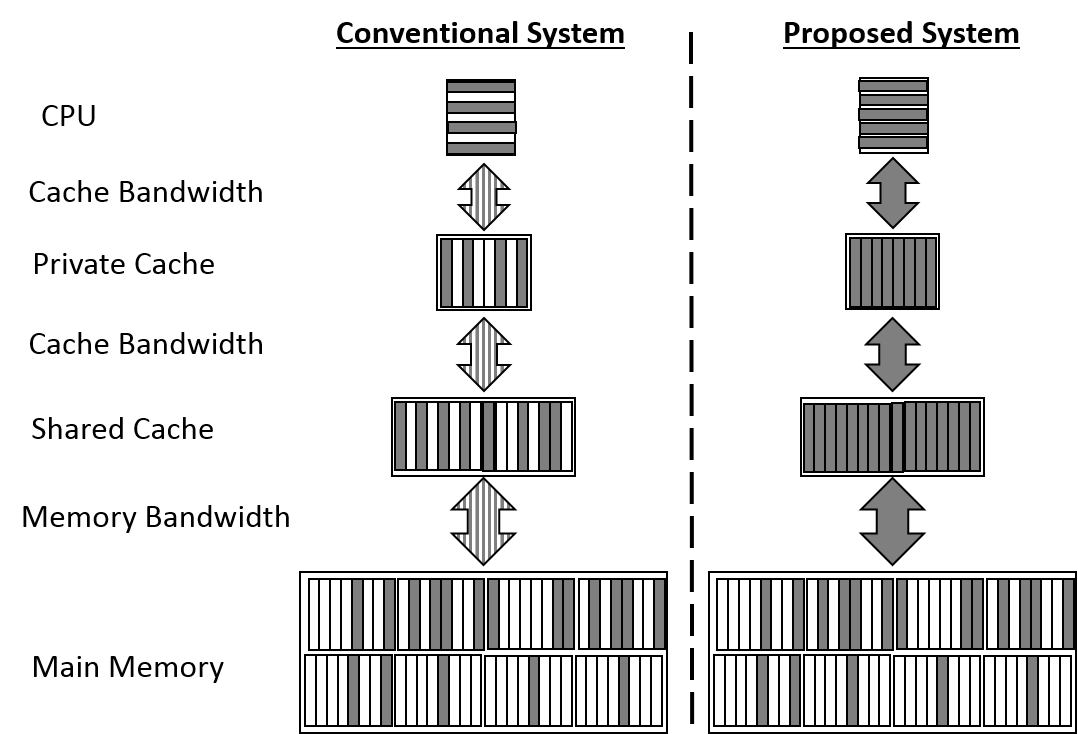
\includegraphics[width=3.4in]{Figures/system-comparison.png}
\caption{Processor and memory system utilization of sparse (white) and non-sparse (shaded) data.}
\label{fig:system-compare}
\end{figure}

Our proposed optimizations can improve DNN training peformance and scalability in three ways.  First, by eliminating computations on useless data while processing a training example, more iterations over the data set can be completed within a time budget (e.g., a week), which can improve model quality.  Second,  memory system  bandwidth is a key bottleneck for {\it data-parallelism} within a machine (i.e., processing multiple examples at once using multiple CPU cores). By reducing the bandwidth utilization for each example, data-parallelism can scale training throughput more effectively.  Finally, a standard approach for fitting big DNN models into the last level cache is partitioning the model across multiple machines to exploit the aggregate cache capacity (a.k.a., {\it model-parallelism}). By reducing the cache consumption of a model partition, our techniques can increase the per-machine partition size and reduce the number of machines required to achieve a target training throughput, reducing model parallelism costs. 

Prior software~\cite{Eisenstat82, IntelSparseMatrix} and hardware~\cite{Carter99, Srinidhi12, Fowers13} approaches for sparse matrix-vector multiplications are less effective for DNN training for two reasons.  First, those techniques assume that sparsity exists only in matrices but not in vectors, whereas in DNN training both matrices and vectors can be sparse.  Second, those techniques assume that the sparse data structures are static, so that the cost of constructing a sparse representation is amortized over many uses.  However, the matrices and vectors in DNN training change for each training example, thus representation cost is incurred repeatedly, hurting performance. 

Our approach consists of processor and memory system techniques for reducing sparse data computation overheads.  Our processor extensions are based on ``zero-optimizable'' instructions, which are arithmetic instructions (e.g., multiplication) whose results and side effects are pre-determined when an input operand is a zero. Our optimizations exploit zero-optimizable instructions to reduce execution cycles and processor resource pressure.  Our memory system extensions efficiently track zero data at cache line granularity to avoid the storage and bandwidth costs of zero cache lines.  Our approach is transparent to software and therefore benefits existing binaries. 

We evaluate our proposed hardware extensions in a simulation environment using real-world DNN training workloads for image recognition. The results show significant improvements in training time in single threaded, multi-threaded, and model-parallelism scenarios.

This paper makes the following contributions.
\begin{itemize}

\item We propose hardware techniques for improving the performance and scalability of DNN training by reducing computational requirements of sparse data computations, without requiring software changes. 
\item We study the impact of sparse data on computation in a real-world DNN training for an image recognition task. 
\item We present a detailed design of our proposed hardware extensions, which add negligible logic on the critical path of processor execution and memory accesses. 
\item We quantitatively evaluate how our optimizations improve DNN training peformance and scalability using standard image recognition workloads. 

\end{itemize}

The rest of the paper is organized as follows.  Section~\ref{sec:background} provides background on DNN and DNN training.  Section~\ref{sec:sparse_dnn_training} studies spare data computations in DNN training.  Our processor optimizations are described in Section~\ref{sec:processor_opt}, while our cache optimizations are described in Section~\ref{sec:cache_opt}.  We present our evalutation results in Section~\ref{sec:eval}, review related work in Section~\ref{sec:related},  and conclude in Section~\ref{sec:conclude}.


